% Intro

% Purpose
The purpose of this section is to study the performance characteristics of the \textit{memtier} clients and \textit{memcached} servers. \\
% Experimental setup
The experimental setup is as follows: We let each experiment run for 80s and each experiment is repeated 3 times. The standard deviation of a specific metric is computed over those repetitions and shown as red error bars in the plots. Note that if the standard deviation is very small, one might not be able to see the red error bars in the plots. Throughput and response time are based on the output of \textit{memtier}, whereas other metrics like the CPU utilization are based on the output of \textit{dstat}. 

\subsection{One Server}
% setup description
In this setup we have 3 memtier instances (each installed on a single VM) connected to a single memcached instance. The overview of the experiment parameters is given in the following table:
\begin{center}
	\scriptsize{
		\begin{tabular}{|l|c|}
			\hline Number of servers                & 1                        \\ 
			\hline Number of client machines        & 3                        \\ 
			\hline Instances of memtier per machine & 1                        \\ 
			\hline Threads per memtier instance     & 2                        \\
			\hline Virtual clients per thread       & \{2,4,8,16,24,32,40\} \\ 
			\hline Workload                         & Write-only and Read-only \\
			\hline Repetitions                      & 3                        \\ 
			\hline 
		\end{tabular}
	} 
\end{center}

% plots
\begin{figure}[H]
   \begin{minipage}{0.48\textwidth}
     \centering
     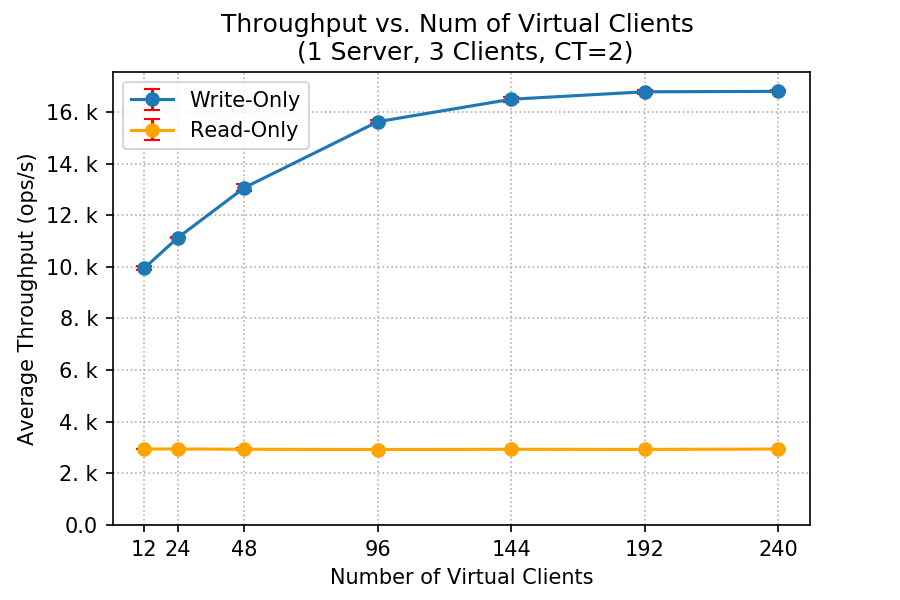
\includegraphics[width=1\linewidth]{figures/1_BaselineWithoutMW/one_server/one_server_mem_tp_2018-10-21_20h12.png}
     \caption{Average throughput.}\label{one_server_tp}
   \end{minipage}\hfill
   \begin{minipage}{0.48\textwidth}
     \centering
     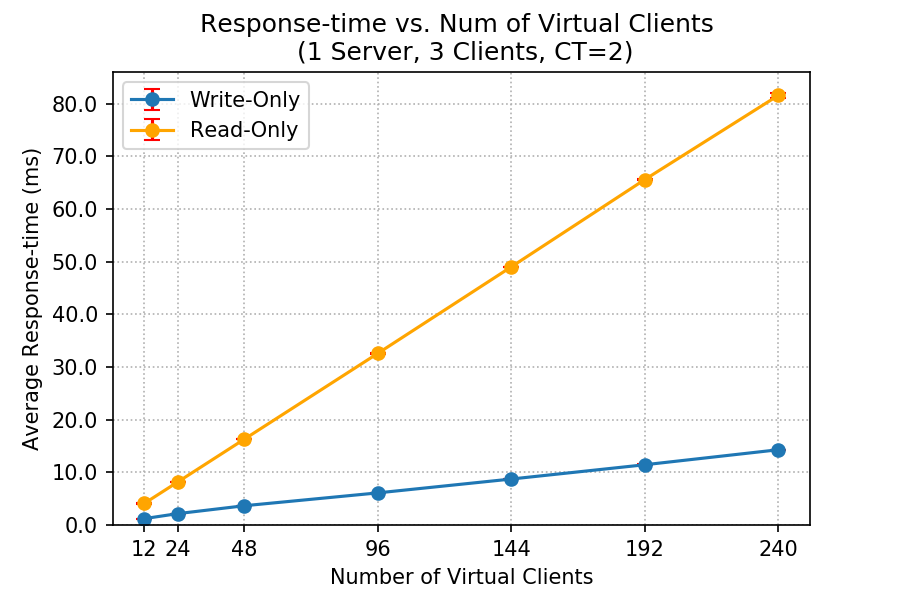
\includegraphics[width=1\linewidth]{figures/1_BaselineWithoutMW/one_server/one_server_mem_rt_2018-10-21_20h12.png}
     \caption{Average response time.}\label{one_server_rt}
   \end{minipage}
\end{figure}
The throughput as a function of virtual clients for read-only and write-only workloads is given in Figure \ref{one_server_tp}, whereas the response time as function of virtual clients for read-only and write-only workloads is given in Figure \ref{one_server_rt}. 

% explanation
% interactive law
The interactive response time law relates throughput and response time in a closed system. It states that $R=N/X-Z$ with response time $R$, throughput $X$, think time $Z$ and $N$ number of clients. $Z$ is often assumed to be zero. The interactive law was checked and holds. Note that for the remaining chapters, the interactive law will be checked for all throughput and response time plots, and unless explicitly stated otherwise, it can be assumed to hold. 

% write throughput: where does memcached saturate, why (what’s the bottleneck)? 
% -> show CPU utilisation plot (dstat) (at 100 percent utilisation) 
If we look at the throughput in Figure \ref{one_server_tp}, we can see that for write-only workloads the system saturates at around $144$ virtual clients because after that the throughput flattens. The CPU utilization plot of the memcached server, which can be seen in Figure \ref{cpu_utilization_one_server}, shows that the CPU is the bottleneck here because it almost reaches full utilization at around the saturation point. 

\begin{figure}[H]
    \begin{minipage}{0.48\textwidth}
        \centering
	    \includegraphics[scale=0.48]{figures/1_BaselineWithoutMW/one_server/dstat_server_cpu_ratio_1:0_2018-10-21_20h12.png}
	    \caption{CPU utilization of a server VM during write-only workload.}
	    \label{cpu_utilization_one_server}
    \end{minipage}\hfill
    \begin{minipage}{0.48\textwidth}
        \centering
	    \includegraphics[scale=0.48]{figures/1_BaselineWithoutMW/one_server/dstat_server_netsend_ratio_0:1_2018-10-21_20h12.png}
	    \caption{Outbound network activity of a server VM during read-only workload.}
	    \label{outbound_net_activity_one_server}
    \end{minipage}
\end{figure}

% read throughput: where does memcached saturate, why (what’s the bottleneck)? 
% network bandwidth, figure out network bandwidth with iperf and then actually used bandwidth with dstat.
% (server upload bandwidth at 12Mbps which is max with  iperf) 
The throughput for read-only workloads stays at the same level during the whole experiment. This indicates that the network bandwidth might be a bottleneck here. In order to confirm this, we first we need to check the maximum outbound network bandwidths for clients and servers. This is done with \textit{iperf}, the results can be seen in the following table: 

\begin{center}
	\begin{tabular}{|l|c|}
	    \hline    & Maximum outbound network bandwidth          \\
		\hline Server VM  & 12.6 MB/s           \\ 
		\hline Client VM & 25 MB/s           \\ 
		\hline 
	\end{tabular}
\end{center}

Now that we know the maximum outbound network bandwidth, we can check the actually used network bandwidth. Figure \ref{outbound_net_activity_one_server} shows that indeed the network activity of memcached server is at its limit and thus the bottleneck of read-only workloads. That the network send activity does not stay perfectly at 12.6 MBps I attribute to noise in the cluster. We can compute the maximal throughput based on the maximal bandwidth of the server to support our claim: A single response from the server is around 4kB because it contains a single value corresponding to a key. Thus if we divide 12.6 MBps by 4kB, we get around 3k requests per second which is exactly what we measured. Saturation is already reached for the lowest number of clients which is why we don't observe under-saturation. 

% response time
Finally we look at the response times in Figure \ref{one_server_rt}. We observe that for read-only workloads the response-time grows faster than for write-only workloads. This makes sense because of the lower throughput for the read-only workloads. \\

\subsection{Two Servers}

% setup description
In this setup we have 2 memtier instances (both run on the same VM), each of which is connected to a single memcached instance. Each memcached instance is installed on a separate VM, i.e. we have two server VMs in total. The overview of the experiment parameters is given in the following table: 
\begin{center}
	\scriptsize{
		\begin{tabular}{|l|c|}
			\hline Number of servers                & 2                        \\ 
			\hline Number of client machines        & 1                        \\ 
			\hline Instances of memtier per machine & 2                        \\ 
			\hline Threads per memtier instance     & 1                        \\
			\hline Virtual clients per thread       & \{1,4,8,16,24,32,40\}        \\ 
			\hline Workload                         & Write-only and Read-only \\
			\hline Repetitions                      & 3              \\ 
			\hline 
		\end{tabular}
	} 
\end{center}

% plots
The throughput as a function of virtual clients for read-only and write-only workloads is shown in Figure \ref{two_server_tp}, whereas the response time as function of virtual clients for read-only and write-only workloads is shown in Figure \ref{two_server_rt}. 
% data: [2018-12-06_10h49]
\begin{figure}[H] % [!htb]
   \begin{minipage}{0.48\textwidth}
     \centering
     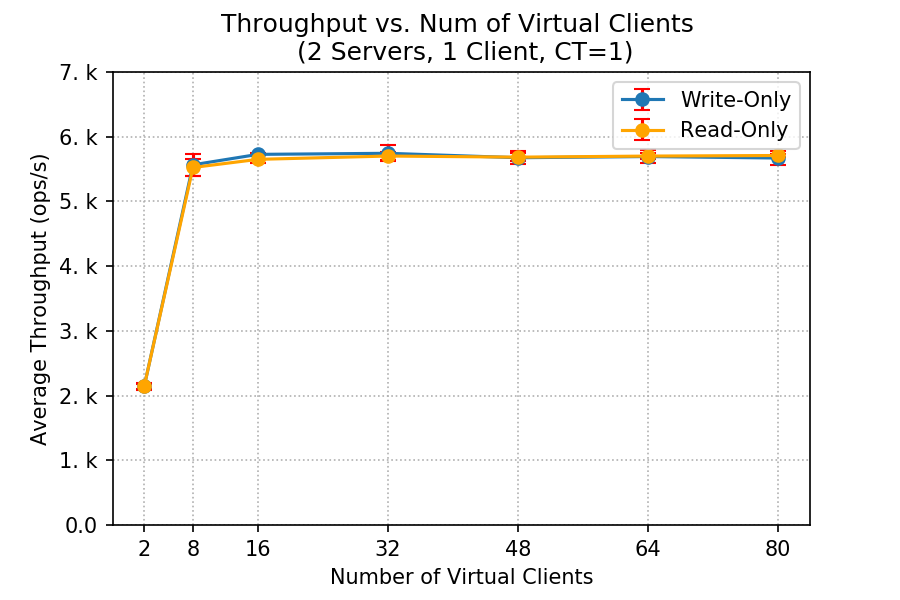
\includegraphics[width=1\linewidth]{figures/1_BaselineWithoutMW/two_servers/two_servers_mem_tp_2018-12-06_10h49.png}
     \caption{Average throughput.}\label{two_server_tp}
   \end{minipage}\hfill
   \begin{minipage}{0.48\textwidth}
     \centering
     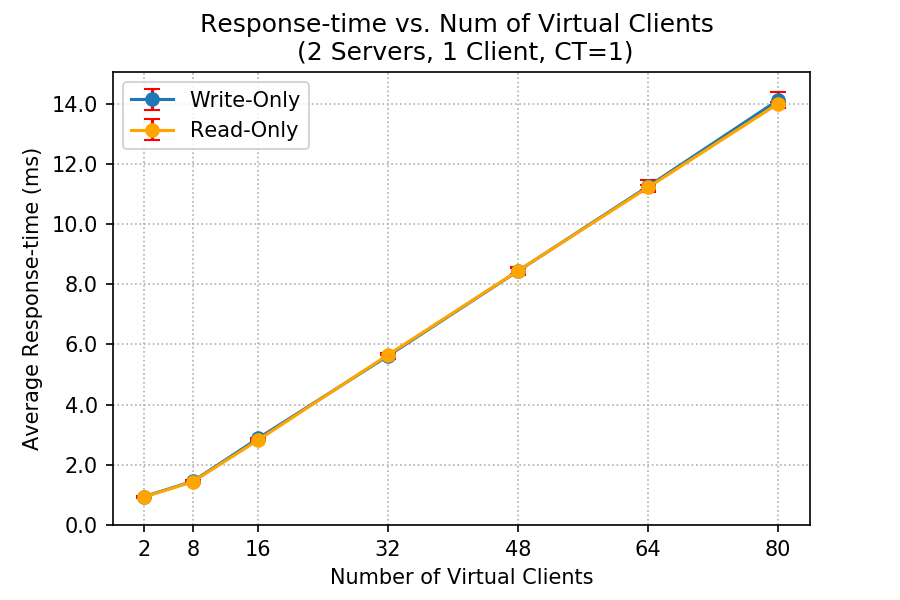
\includegraphics[width=1\linewidth]{figures/1_BaselineWithoutMW/two_servers/two_servers_mem_rt_2018-12-06_10h49.png}
     \caption{Average response time.}\label{two_server_rt}
   \end{minipage}
\end{figure}

% explanation
% interactive law
First of all the interactive law was checked and holds. 
% write throughput: where does memcached saturate, why (what’s the bottleneck)? 
% -> show outbound bandwidth at memtier (at 23MBps)
For write-only workloads the system  already saturates at $8$ virtual clients because from this point on, the throughput flattens and the response time starts increasing significantly, as it can be seen in Figures \ref{two_server_tp} and \ref{two_server_rt}. The bottleneck here is the outbound network bandwidth of the client VM. This can be seen in Figure \ref{outbound_client_net_activity_two_servers} which shows that the maximum bandwidth of $25$ MB/s (checked with \textit{iperf}) for the client VM is reached. The network send activity not being perfectly at $25$ MBps I attribute to noise on the cluster.

% data: [2018-12-06_10h49]
\begin{figure}[H]
	\begin{minipage}{0.48\textwidth}
	    \centering
	    \includegraphics[scale=0.48]{figures/1_BaselineWithoutMW/two_servers/dstat_client_netsend_ratio_1:0_2018-12-06_10h49}
	    \caption{Outbound network activity of the client VM.}
	    \label{outbound_client_net_activity_two_servers}
   \end{minipage}\hfill
   \begin{minipage}{0.48\textwidth}
        \centering
	    \includegraphics[scale=0.48]{figures/1_BaselineWithoutMW/two_servers/dstat_server_netsend_ratio_0:1_2018-12-06_10h49.png}
	    \caption{Outbound network activity of a server VM.}
	    \label{outbound_server_net_activity_two_servers}
   \end{minipage}
\end{figure}

%read throughput: where does throughput reach saturation? bottleneck?
%->outbound bandwidth at server (12MBps)
For read-only workloads the system also saturates at $8$ virtual client for the same reasons, as can be seen in Figures \ref{two_server_tp} and \ref{two_server_rt}. The bottleneck here is also the outbound network bandwidth, but now of the server VMs and not the client VM. This can be seen in Figure \ref{outbound_server_net_activity_two_servers}, which shows that the maximum bandwidth of $12.6$ MB/s (checked with \textit{iperf}) for the server VM is reached at $8$ virtual clients, which is exactly the saturation point of the read-only workload. 

% general remark: set size resp. get response size -> bottleneck
Note that those results also make sense because for the read-only workloads the responses contain $4$ kB values, which mainly affect the outbound bandwidth at the server, whereas the requests just contain the keys which require a few bytes. On the other hand, for the write-only workloads we have the opposite case, i.e. the requests contain the $4$ kB values, which leads to an outbound bandwidth problem at the clients and the responses just contain a status code of a few bytes. 

\subsection{Summary}

\begin{center}
	{Maximum throughput of different VMs.}
	\begin{tabular}{|l|p{2.5cm}|p{2.5cm}|p{4cm}|}
		\hline                        & Read-only workload & Write-only workload & Configuration giving maximum throughput \\ 
		\hline One memcached server   &  2'924 reqs/s & 15'624 reqs/s & 12 clients for read-only, 96 clients for write-only        \\ 
		\hline One load generating VM & 5'897 reqs/s & 5'976 reqs/s   & 8 clients for read-only and write-only           \\ 
		\hline 
	\end{tabular}
\end{center}
The table above shows the maximum throughput for both experiments. Note that when determining the maximum throughput of the system, we take the response time and how it is affected by the increase in load into consideration. For the one server case and write-only workload, going from 96 to 144 clients increases the throughput by $5.6 \%$ while increasing the response time by $30 \%$, which is why we chose the 96 client configuration. For the one server case and read-only workload, we choose the lowest number of clients because the throughput remains the same while the response time increases with more clients. For the two server case and write-only workload, going from 8 to 16 clients increases the throughput by $2.8 \%$, while increasing the response time by $50 \%$ and similar numbers for the read-only workload. 

% one server
For the one server experiment, we tested the limits of a single server. For write-only workloads the bottleneck is its CPU and for read-only workloads the bottleneck is its outbound network bandwidth, which is plausible because for the writes it has to process a lot of big requests, and for the reads it has to send back big responses. The reason that reads have a much smaller throughput than the writes is that the server only has a $12$ MBps outbound network bandwidth, which is a much more limiting factor than the CPU for the writes. 

% two server
For the two server experiment, we tested the limits of a single client. For both kind of workloads the bottleneck is the network bandwidth and the throughput is very similar, which I guess is just a coincidence based on the maximal outbound network bandwidth of the client and the server VM. 

% Comparison
Comparing the read-only throughput of the experiments, we observe that doubling the number of servers also roughly doubles the read-only throughput on average. This is because in the one server case we did not provide enough server bandwidth resources. 
Comparing the write-only throughput of the experiments, we observe that the one server case has roughly $2-3$ times the throughput of the two server case. This is because in the two server case we did not provide enough client bandwidth resources. 

% Take-away messages about behavior of clients and servers
The conclusion is that the server and client resources need to be carefully selected for the performance analysis of the middleware. If we want the observe the bottlenecks of the middleware, we need to provide enough resources such that we are not limited for example by the network bandwidth or CPU of the server or client VMs. 